\vspace{10pt}

{\centering\subsection*{郭睿:《小王子》读后感}}

\addcontentsline{toc}{subsection}{郭睿:《小王子》读后感}

\renewcommand{\leftmark}{郭睿:《小王子》读后感}

\begin{figure}[htbp]

\centering

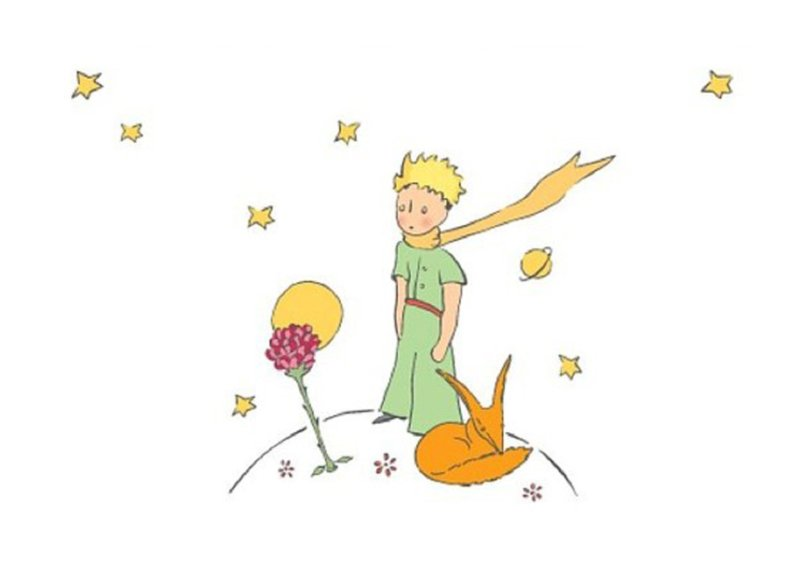
\includegraphics[width = .5\textwidth]{./ch/31.jpg}

\end{figure}





我喜欢看一些童话、冒险的书,因为有有趣的地方。

《小王子》是童话书,书里面有很多内容。《小王子》这个书名直接让我们一目了然。主角是小王子,但还有一位主角是小公主。

小王子去过许多星球,别的星球上都有一位国王,而小王子却没有星球,最后小王子住在小公主家的隔壁。

小王子是一位飞行员,小王子去的每一个的行为让我感到小王子实事求是。而小公主是一位善良、有目标、有责任的人。小公主每天学习,没有一次不学。

小王子让我学到了怎么才能实事求是。小公主让我学到了怎么有目标,怎样才能造就成功的希望!

点评:给出了读书理由,并说出了看到的故事情节,对主人公进行了评价,最后还说出了给自己的启发。无论文字如何简单,开始写是一个重大的转变。写能梳理思路,并锻炼用自己的话呈现出看到的内容和自己的理解,这是一种印象更深刻的阅读方式。





\vspace{10pt}



作者:六(4)班 郭睿

指导老师:于鸿锦

投稿:2021年5月1日

发表:2021年5月2日


                



\vspace{10pt}

\hline



